\documentclass{article}
\usepackage[utf8]{inputenc}
\usepackage{caption}
\usepackage{graphicx}
\usepackage{courier} %% Sets font for listing as Courier.
\usepackage{listings, xcolor}
\lstset{
tabsize = 4, %% set tab space width
showstringspaces = false, %% prevent space marking in strings, string is defined as the text that is generally printed directly to the console
numbers = left, %% display line numbers on the left
commentstyle = \color{green}, %% set comment color
keywordstyle = \color{blue}, %% set keyword color
stringstyle = \color{red}, %% set string color
rulecolor = \color{black}, %% set frame color to avoid being affected by text color
basicstyle = \small \ttfamily , %% set listing font and size
breaklines = true, %% enable line breaking
numberstyle = \tiny,
}

\title{Gesture Based UI Project}
\author{Emmanuel Osabuehien (G00373559)}
\date{\today}

\begin{document}

\maketitle

\section{Introduction}

\section{Purpose of the application}

\subsection{What Is The Game}

The purpose of this game is to learn, understand, explain and implement the use of voice commands and gesture control with various technology, for the voice commands we will be using Cortana and for the gesture control we will be using Myo Armband. For my application, I decided to recreate the classic arcade game 'Space Invaders' with the programming language Java, to create our we used an integrated development environment (IDE) known as 'Eclipse'. The Game uses gesture control to control the movement (moving left and right) and actions (shooting bullets) of the player and uses voice commands to control actions of the game where you can start, pause, resume and reset the game.

\begin{figure}[h]
  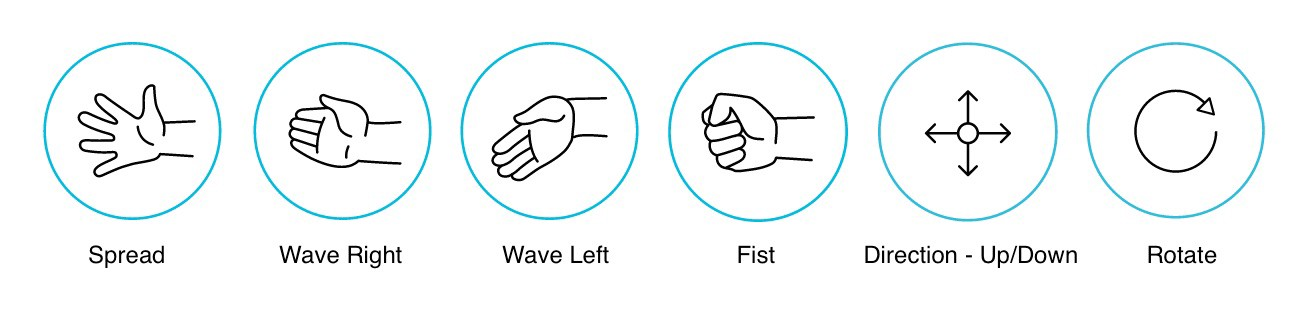
\includegraphics[width=\textwidth]{img/gestures.jpg}
  \centering
  \caption{Example of Different Gesture Controls}
  \label{fig: Myo Armband Gesture Controls}
\end{figure}

\subsection{Design Of The Game}

The design of the game should look as follows:

\subsection{How To Run Application}

For our application, we have a Myo Script where have a function that connects the gesture controls to our application where if it locates the title of the applicatin 'GUI Project' it will return true, the code is as follows:

\begin{lstlisting}[language = Java , frame = trBL , firstnumber = last , escapeinside={(*@}{@*)}]
function onForegroundWindowChange(app, title)
    if title == "GUI Project" then
        reference = getRoll()
        return true
    end 
end
\end{lstlisting}

\subsection{Voice Commands}

When implementing voice commands, I used various jar files that I researched and found online to complete the use of voice controls, the main jar files known as 'Voce' that can be used by both Java and C++.\\ \\

\begin{lstlisting}[language = Java , frame = trBL , firstnumber = last , escapeinside={(*@}{@*)}]
public <String> = [start | reset | stop | continue ];
\end{lstlisting}
\\ \\
We set up an array of strings which contain the four voice commands that our game will use which include:

\begin{itemize}
    \item Start: To start the game
    \item Stop: To pause the game
    \item Continue: To resume the game when paused
    \item Reset: To reset the game from the beginning
\end{itemize}

\section{Gestures identified as appropriate for this application}

Unfortunately my the partner that I originally was working on this project with, decided to sadly leave this course meaning I had full control and freedom to decide how I would incorporate gestures into my application.\\ \\
I was given two different options for hardware when using gesture control, using either the Myo Armband or the Leap Motion Sensor, I researched both pieces of hardware and after completing my research I decided to use the Myo Armband due to it's pre-built gestures which I decided would work great with my concept of the application, the Myo Armband has seven pre-built gestures which include:

\begin{itemize}
    \item Wave Left
    \item Wave Right
    \item Rotate
    \item Spread Fingers
    \item Double Tap
    \item Make Fist
    \item Direction - Up/Down
\end{itemize}
\\ \\
When implementing the gestures into my application, we initially used the spread fingers gesture to control the shooting of the player and the wave left and wave right to control the movement of the player but as we progressed in the development of the project we decided to change this due to different reasons.\\ \\
After using the wave left and wave right gesture to control the movement, this became strenuous to continually have to wave your arms in both directions so we decided to use the rotate gesture instead as it didn't exhaust the user to rotate your hand clockwise and anti-clockwise to move the player from right to left and from left to right.\\ \\
After using the spread fingers gesture to control the shooting of the player, this gesture was not quick to react which meant I had to switch to something else, so I decided to go with the make fist gesture as it reacted on time and was much more precise.

\section{Hardware used in creating the application}

\section{Architecture for the solution}

\section{Conclusions \& Recommendations}

\end{document}
